\documentclass[11pt]{article}
\usepackage[T1]{fontenc}
\usepackage[utf8]{inputenc}
\usepackage{lmodern,microtype}
\usepackage[margin=1.05in]{geometry}
\usepackage{amsmath,amssymb,amsthm,mathtools,bm}
\usepackage{enumitem,graphicx,booktabs,array}
\usepackage{tikz}
\usetikzlibrary{arrows.meta,positioning,calc}
\usepackage[numbers,sort&compress]{natbib}
\usepackage{xurl}
\usepackage[colorlinks=true,linkcolor=blue!45!black,citecolor=blue!45!black,urlcolor=blue!45!black]{hyperref}
\usepackage[capitalise,noabbrev]{cleveref}
\usepackage{bookmark}
\pdfinfoomitdate=1
\pdftrailerid{}
\pdfsuppressptexinfo=15
\input{glyphtounicode}
\input{glyphtounicode-cmex}
\pdfgentounicode=1
\hypersetup{pdftitle={Generalized outer-electron radii of neutral Coulomb atoms},pdfauthor={OpenAI},bookmarksdepth=2}
\newtheorem{theorem}{Theorem}[section]
\newtheorem{proposition}[theorem]{Proposition}
\newtheorem{lemma}[theorem]{Lemma}
\newtheorem{corollary}[theorem]{Corollary}
\theoremstyle{definition}
\newtheorem{definition}[theorem]{Definition}
\theoremstyle{remark}
\newtheorem{remark}[theorem]{Remark}
\numberwithin{equation}{section}
\newcommand{\R}{\mathbb R}
\newcommand{\C}{\mathbb C}
\newcommand{\N}{\mathbb N}
\newcommand{\E}{\mathbb E}
\newcommand{\Prob}{\mathbb P}
\newcommand{\dd}{\,\mathrm d}
\newcommand{\eps}{\varepsilon}
\newcommand{\1}{\mathbf1}
\newcommand{\FoundationBinding}{Lemma~2.5}
\newcommand{\FoundationMonotonicity}{Lemma~2.1}
\newcommand{\FoundationConstants}{Equation~(1.3)}
\newcommand{\FoundationOffset}{Proposition~12.3}
\newcommand{\FoundationCounts}{Corollary~4.9}
\newcommand{\FoundationDeficit}{Lemma~12.2}
\newcommand{\FoundationComparison}{Proposition~10.1}
\newcommand{\FoundationIntermediate}{Proposition~11.2}
\newcommand{\FoundationObservations}{Lemma~5.1 and Section~10.1}
\newcommand{\EnergyProfile}{Section~5}

\DeclareMathOperator{\supp}{supp}
\DeclareMathOperator{\dist}{dist}
\setlength{\emergencystretch}{1.5em}
\setlist[enumerate]{itemsep=.3em,topsep=.5em}
\setlist[itemize]{itemsep=.2em,topsep=.4em}
\title{Generalized outer-electron radii of neutral Coulomb atoms}
\author{OpenAI}
\date{September 24, 2026}
\begin{document}
\maketitle
\begin{abstract}
We prove the radius part of the generalized ionization conjecture for
neutral nonrelativistic Coulomb atoms with two spin states. For every
choice of ground states, the upper and lower large-nuclear-charge limits
of the radius defined by an expected exterior electron mass $m$ are both
asymptotic to $(81\pi^2/2)^{1/3}m^{-1/3}$ as $m$ tends to infinity.
\end{abstract}
\setcounter{tocdepth}{1}
\tableofcontents
\section{Introduction}\label{sec:introduction}

The ionization problem asks how the outer electrons of an atom behave
as its nuclear charge increases.  The generalized ionization conjecture
predicts universal asymptotics for both ionization energies and radii
defined by a prescribed exterior electron mass.  We resolve its radius
part positively for the full correlated two-spin Schr\"odinger model,
using the conditional screening and propagation estimates of
\cite{OuterRadius}.

\subsection{Statement of the result}

In atomic units, for each integer $Z\ge1$ let
\begin{equation}\label{intro:hamiltonian}
 H_Z=\sum_{i=1}^{Z}\left(-\frac12\Delta_{x_i}-\frac{Z}{|x_i|}\right)
       +\sum_{1\le i<j\le Z}\frac1{|x_i-x_j|}
 \quad\hbox{on }\bigwedge^ZL^2(\R^3;\C^2).
\end{equation}
The operator is associated with its usual closed, bounded-below quadratic
form.  Let $\Psi_Z$ be any normalized ground state and let its spin-summed
one-electron density be
\begin{equation}\label{intro:density}
 \rho_{\Psi_Z}(x)
 =Z\sum_{\sigma_1,\ldots,\sigma_Z\in\{1,2\}}
   \int_{\R^{3(Z-1)}}
   |\Psi_Z(x,\sigma_1;x_2,\sigma_2;\ldots;x_Z,\sigma_Z)|^2
   \dd x_2\cdots\dd x_Z.
\end{equation}
For $Z=1$ the integral is absent.  Thus $\int\rho_{\Psi_Z}=Z$.
For integers $1\le m<Z$, define
\begin{equation}\label{intro:radius}
 R_m(\Psi_Z)=\inf\left\{r\ge0:
               \int_{|x|>r}\rho_{\Psi_Z}(x)\dd x\le m\right\}.
\end{equation}
This is a radius in the neutral atom: $m$ specifies the expected electron
mass outside the sphere.  The state itself still has $Z$ electrons.

\begin{theorem}[Generalized ionization conjecture: radii]\label{intro:main}
Set $b_{\mathrm{TF}}=(81\pi^2/2)^{1/3}$.  For every choice of normalized
neutral ground states $(\Psi_Z)_{Z\ge1}$ of \eqref{intro:hamiltonian},
\begin{align}
 \lim_{m\to\infty}m^{1/3}
       \left[\limsup_{\substack{Z\to\infty\\ Z>m}}R_m(\Psi_Z)\right]
       &=b_{\mathrm{TF}},\label{intro:limsup}\\
 \lim_{m\to\infty}m^{1/3}
       \left[\liminf_{\substack{Z\to\infty\\ Z>m}}R_m(\Psi_Z)\right]
       &=b_{\mathrm{TF}}.\label{intro:liminf}
\end{align}
All limits are over integers.  The inner limits hold $m$ fixed; no
convergence in $Z$ at a fixed $m$ is assumed.
\end{theorem}

The statement is uniform over all choices in each ground eigenspace.
Neither the state nor its density is assumed to be spherically symmetric.
Existence of these ground states, in the same form and spin convention,
follows from the strict binding statement in
\cite[\FoundationBinding]{OuterRadius}.

\subsection{History and scope}

The Thomas--Fermi approximation became a rigorous description of the
leading energy and scaled bulk density through the work of Lieb and
Simon \cite[Theorems~III.1 and~III.3]{LiebSimon1977}.
A neutral atom has bulk length scale
$Z^{-1/3}$, while the radius in \eqref{intro:radius}, at fixed $m$,
concerns only the fraction $m/Z$ of its mass.  Convergence of the bulk
density therefore leaves this outer-electron question unresolved.
For the full quantum model, Seco, Sigal, and Solovej obtained a
quantitative lower bound on the radius containing all but one expected
electron \cite[Theorem~3]{SecoSigalSolovej1990}.  This concerns the same
expected-tail notion of radius, but its lower bound still decays with $Z$
and does not determine a universal outer-radius law.

Solovej's unrestricted Hartree--Fock theorem established the universal
outer-radius asymptotic with the same constant as in
\cref{intro:main} \cite[Definition~1.2 and Theorem~1.5]{Solovej2003}.
Its proof controls screened potentials on successively larger exterior
regions \cite[Sections~10--13]{Solovej2003}, uniformly in the chosen
Hartree--Fock minimizer.  The generalized ionization conjecture for the
full Schr\"odinger model explicitly retains both upper and lower
large-$Z$ limits \cite[Section~3, Equation~(2)]{Solovej2016}.
The order of limits in \cref{intro:main} is precisely this formulation.
Sharp radius estimates were subsequently obtained for minimizers in
Thomas--Fermi--Dirac--von Weizs\"acker theory
\cite[Theorem~1.3]{FrankNamVanDenBosch2018} and for power density-matrix
functionals \cite[Theorem~3]{Kehle2017}.  These are results for distinct
approximate variational models, not for arbitrary correlated
Schr\"odinger ground states.

The limiting profile has its own earlier analytic theory.  Lieb and
Simon proved directional Sommerfeld asymptotics for neutral
Thomas--Fermi systems \cite[Theorem~IV.10]{LiebSimon1977}.
Solovej's later comparison estimate explicitly allows nonradial
solutions \cite[Lemma~4.4 and Remark~4.5]{Solovej2003}; the homogeneous
rigidity statement used here is a consequence of that estimate.
We give a short dilation proof in \cref{prof:rigidity}.  The additional
task is to obtain such a profile from correlated quantum ground states
and then recover their expected exterior mass.

For the full model, the foundation companion already bounds above and
below, uniformly in $Z$ and the neutral ground state, the radius leaving
one half of an electron in expected exterior mass
\cite[Theorem~1.2]{OuterRadius}.  The present theorem identifies the
sharp coefficient as the prescribed exterior mass tends to infinity.
The same companion supplies the conditional density comparisons and
positive intermediate subsolutions used for this passage.
Section~\ref{sec:inputs} defines their common observations
and smoothing conventions; Appendix~\ref{sec:interface} records the
provider results and the order of parameter choices.
The intermediate-scale compactness strategy also appears in the
energy companion \cite[\EnergyProfile]{EnergyPart}.
That is a shared method: the proof here uses only the foundation
estimates and establishes its own neutral-profile and expected-tail
arguments.

\subsection{Proof and reusable ingredients}

The limiting neutral Thomas--Fermi model explains both the rescaling and
the radius coefficient.  Its density $\varrho$ and screened field $F$
satisfy, away from the nucleus,
\begin{equation}\label{intro:constants}
 \varrho=k(F_+)^{3/2},\qquad \Delta F=4\pi\varrho,
 \qquad k=\frac{2^{3/2}}{3\pi^2},\qquad t_+=\max(t,0).
\end{equation}
Here $k$ corresponds to two spin states and kinetic operator $-\Delta/2$
\cite[\FoundationConstants]{OuterRadius}.  Since
$\Delta|x|^{-4}=12|x|^{-6}$, the positive radial homogeneous solution is
$F_*(x)=A_*|x|^{-4}$, with
\begin{equation}\label{intro:sommerfeld}
 A_*:=\left(\frac{12}{4\pi k}\right)^2=\frac{81\pi^2}{8},
 \qquad \rho_*(x):=kA_*^{3/2}|x|^{-6}\quad(x\ne0).
\end{equation}
Its exterior mass is
\[
 \int_{|x|>r}\rho_*(x)\dd x=4A_*r^{-3}
       =b_{\mathrm{TF}}^3r^{-3},
\]
so prescribing mass $m$ gives radius $b_{\mathrm{TF}}m^{-1/3}$.
These are equations for the limiting model, not identities for the
quantum density $\rho_{\Psi_Z}$.

To reach this model from a quantum state, we add small independent errors
to the electron positions and condition on the resulting unordered
observations.  Conditionally averaging smooth unit-mass packets around
the electron positions gives a density; subtracting its Coulomb potential
from the nuclear potential gives the screened field.  At an intermediate
radius $s$, we rescale this field by $s^4$ and the density by $s^6$.
The comparison estimate gives a pointwise Thomas--Fermi relation on
larger and larger rescaled annuli.  Two difficulties remain: the field
has only an upper bound, and the total rescaled electron mass can diverge.
Exact neutrality makes its spherical mean nonnegative.  The upper bound
then controls the full local $L^1$ norm, so harmonic interior estimates
give compactness even for these signed fields.

The intermediate subsolutions transfer a strictly positive lower bound
to each limit.  Dilation compactness and contact at approximate extrema
then identify the field as the homogeneous Sommerfeld profile, without
assuming radiality.  The compactness and rigidity criteria are stated
separately in \cref{prof:compactness,prof:rigidity}.

Finally, a conditional profile must be related to the expected mass
defining \eqref{intro:radius}.  A localized $L^2$ count estimate removes
the exceptional observations; shrinking packet supports remove the
smoothing; and a separate dyadic estimate controls the distant tail.
The resulting mass asymptotic, proved along every admissible sequence,
gives both iterated limits by a finite-threshold argument in $Z$.

The proof follows these steps in order.  Section~\ref{sec:scales}
selects observations on expanding annuli, Section~\ref{prof:section}
identifies the limiting field, and Section~\ref{sec:tails} passes to
expected raw counts and proves the radius limits.

\subsection{Notation}

Write $K(x)=|x|^{-1}$, $V=ZK$, and $f(t)=4\pi k(t_+)^{3/2}$.
Constants $C,c>0$ may change from line to line; their permitted
dependencies will be specified.
Expectations include the spin sum and any stated auxiliary randomness.
For the raw spatial configuration of $\Psi_Z$, antisymmetry gives
\begin{equation}\label{intro:count-density}
 \E\#\{i:x_i\in A\}=\int_A\rho_{\Psi_Z}(x)\dd x.
\end{equation}
All finite-system radial boundary spheres have probability zero.

\section{Conditional screening inputs}\label{sec:inputs}

We define one family of screened conditional fields and state the
foundation estimates used to study it.  Their complete proofs are in
\cite{OuterRadius}; Appendix~\ref{sec:interface} collects the parameter
order and provider map.  All constants and thresholds below are uniform
over neutral ground states.

\subsection{Energy offset and count bounds}

For a fixed nuclear charge $Z$, let $E_n=E_n(Z)$ be the bottom of the
$n$-electron Hamiltonian with the same kinetic and spin conventions as
\eqref{intro:hamiltonian}, and put $E=\inf_{n\ge0}E_n$.
A normalized state has offset $\delta$ if its energy is at most $E+\delta$.

\begin{proposition}[Uniform offset and raw counts]\label{inp:energy-counts}
There are constants $D_0,Z_0<\infty$ such that every normalized neutral
ground state with $Z\ge Z_0$ has offset at most $D_0$.
For every fixed $0<\alpha<\beta<\infty$ and every $u>0$, its raw
electron configuration satisfies
\begin{equation}\label{inp:counts}
 \begin{aligned}
 \left\|\#\{i:\alpha u<|x_i|<\beta u\}\right\|_{L^2(\Prob)}
 &\le C_{\alpha,\beta}
       \bigl(\max\{u^{-3},1\}+\sqrt{D_0u}\bigr),\\
 \E\#\{i:|x_i|>1\}&\le C(1+\sqrt{D_0}).
 \end{aligned}
\end{equation}
\end{proposition}

\begin{proof}
Monotonicity of the sector energies
\cite[\FoundationMonotonicity]{OuterRadius} and the bounded offset of the
$(Z-1)$-electron sector \cite[\FoundationOffset]{OuterRadius} give
$E\le E_Z\le E_{Z-1}\le E+C$.  Take $D_0=C$.
The first assertion in \eqref{inp:counts} is
\cite[\FoundationCounts]{OuterRadius}.  The second follows from
\cite[\FoundationDeficit]{OuterRadius} with $t=4$, since neutrality gives
\[
 \E\#\{i:|x_i|>1\}=Z-\E\#\{i:|x_i|<1\}.
\]
Boundary spheres have zero probability, so either convention for
annular endpoints gives the same estimates.
\end{proof}

\subsection{One family of observations and packets}

The comparison estimate concerns a smoothed density conditioned on noisy
position observations.  As the observation index increases, we discard
finer observations; the propagation construction uses conditional
averaging over the discarded data.  We use one packet family throughout,
so that comparison and propagation concern the same fields.

Fix a real smooth radial function $g$, supported in the unit ball and
normalized by $\int g^2=1$, and set
$g_t(y)=t^{-3/2}g(y/t)$.  Fix the universal constants
\[
 w=10^{-5},\qquad L=10^5,\qquad 0<c_1<(10L)^{-1}.
\]
Also fix $\eps>0$ sufficiently small for the barrier construction below.
For $0<s<1$ and $Z$ large enough that $2\eps Z^{-1/3}\le s$, define
\begin{equation}\label{inp:observations}
 r_0=\eps Z^{-1/3},\qquad r_j=2^jr_0,\qquad
 J=\max\{j:r_j\le s\},\qquad s/2<r_J\le s.
\end{equation}
For each $j<J$ observe the unordered array
$\{x_i+r_j^{1.01}U_{ji}:1\le i\le Z\}$.  Every Cartesian
coordinate of every $U_{ji}$ is independent, independent of the raw
configuration, and has density
$c_\zeta\exp[-1/(1-u^2)]\mathbf1_{\{|u|<1\}}$.
Let $\mathcal F_j$ retain the arrays with indices $j,\ldots,J-1$;
let $\mathcal F_J$ be trivial.  Thus the sigma-fields decrease with $j$.

For a possible electron center $x$, define the master packets and their
conditional densities by
\begin{equation}\label{inp:packets}
 \begin{gathered}
 d_x=|x|,\qquad \widehat d_x=\max\{d_x,r_0\},\qquad
 t_x=c_1\widehat d_x\min\{\widehat d_x,s\}^{w},\\
 \mathcal K_x(y)=g_{t_x}(y-x)^2,\qquad
 \mu_j(y)=\E\left[\sum_{i=1}^Z\mathcal K_{x_i}(y)
                  \,\middle|\,\mathcal F_j\right],
 \qquad H_j=V-K*\mu_j .
 \end{gathered}
\end{equation}
The upper clamp acts only on the factor raised to $w$.
In particular $t_x\ge c_1r_0^{1+w}>0$, every packet has mass one,
and its support is contained in $B(x,t_x)$.
Unlike the unconditional raw density $\rho_{\Psi_Z}$, the density
$\mu_j$ depends on the observed data and includes packet smoothing.
Section~\ref{sec:tails} removes both operations to recover the expected
raw mass defining the radius.

We use the conditional-integral versions in
\cite[\FoundationObservations]{OuterRadius}: at data of positive marginal density,
integrate against the raw law multiplied by the observation likelihood
and divided by that marginal density.  These versions are jointly
measurable.  For each finite system, every spatial derivative of
$\mu_j$ has a deterministic bound, since the widths have a positive
lower bound.  Almost surely,
\begin{equation}\label{inp:mass-poisson}
 \mu_j\ge0,\qquad \int\mu_j=Z,\qquad
 \Delta H_j=-4\pi Z\delta_0+4\pi\mu_j .
\end{equation}
The remainder $H_j-V$ is continuous and locally Lipschitz even at zero.
For example, splitting the Coulomb potential and its gradient at unit
distance uses boundedness of $\mu_j$ near the singularity and its finite
mass farther away.  The corresponding regularity bounds may depend on
$Z$.  The conditional tower identity for $\mu_j$ holds pointwise in
space; the identity for $H_j$ holds away from the nucleus, and that
for the continuous extension of $H_j-V$ holds everywhere.  Both
identities hold after integration against smooth compactly supported
tests.

\begin{samepage}
\subsection{The inverse comparison}

\begin{proposition}[Conditional comparison]
\label{inp:comparison-prop}
There is a universal $C_{\mathrm{cap}}$ with the following property.
Fix $L_1\ge2$, $0<h_l<h_h<\infty$, and $0<\xi<h_l/16$.
For all sufficiently small $s>0$, depending on these parameters and
$D_0$, and each $j<J$, there is an event in $\mathcal F_j$ whose
complement has probability at most $Cr_j^{25}$, on which, simultaneously
for $r_j\le |y|\le4L_1r_j$ and $h_l\le h\le h_h$,
\begin{equation}\label{inp:comparison}
 \begin{gathered}
 H_j(y)\le C_{\mathrm{cap}}|y|^{-4},\\
 |y|^6\mu_j(y)>kh^{3/2}
       \quad\Longrightarrow\quad |y|^4H_j(y)\ge h-\xi,\\
 |y|^6\mu_j(y)<kh^{3/2}
       \quad\Longrightarrow\quad |y|^4H_j(y)\le h+\xi.
 \end{gathered}
\end{equation}
The probability constant may depend on the fixed comparison
parameters, but $C_{\mathrm{cap}}$ does not.
The estimates are uniform in $Z$, the ground state, $j$, and $J$.
\end{proposition}
\end{samepage}

This is \cite[\FoundationComparison]{OuterRadius}.
The observations and packets in \eqref{inp:observations}--\eqref{inp:packets}
are chosen before $L_1,h_l,h_h,\xi$.  Varying the comparison accuracy or
its annular width therefore does not change the conditional fields.
This common choice is essential when we combine increasingly accurate
comparisons with a single barrier construction.

\subsection{Intermediate subsolutions}

\begin{proposition}[Intermediate subsolutions]
\label{inp:barrier-prop}
For the fixed constants above, there are $B>0$, $C_{\mathrm{inv}}<\infty$,
$s_{\mathrm{bar}}>0$, and a finite integer threshold
$Z_{\mathrm{bar}}(s)$ for every $0<s\le s_{\mathrm{bar}}$, such that
the following holds.  For every $Z\ge Z_{\mathrm{bar}}(s)$ and
every neutral ground state,
\cite[\FoundationIntermediate]{OuterRadius} supplies, at each $0\le j\le J$,
$\mathcal F_j$-measurable functions $u_j,p_j$ satisfying
\begin{equation}\label{inp:barriers}
 \begin{gathered}
 \Delta u_j\ge-4\pi Z\delta_0+
     4\pi\mathbf1_{\{|y|<r_j\}}\mu_j-4\pi p_j+
     \mathbf1_{\{|y|\ge r_j\}}f(u_j)
       \quad\hbox{in }\mathcal D'(\R^3),\\
 B|y|^{-4}\left(1-\frac{r_j}{8|y|}\right)
       \le u_j(y)\le C_{\mathrm{inv}}|y|^{-4}
       \quad (|y|\ge r_j),\\
 p_j\ge0,\qquad \supp p_j\subset\{|y|\le r_j\},\qquad
 \E\int p_j\le C(s^{32}+s^\gamma),\qquad
 \gamma=\frac{19}{2}-3w>0.
 \end{gathered}
\end{equation}
For each finite system and index, $p_j$ is bounded and $u_j-V$ is
continuous and locally Lipschitz through zero.  The constants $B$,
$C_{\mathrm{inv}}$, and $C$ and the thresholds are independent of the
ground state and of the number of dyadic scales.
We enlarge $Z_{\mathrm{bar}}(s)$ to include $Z\ge Z_0$ and $2r_0\le s$.
\end{proposition}

The bound on the expected error is valid at every intermediate index.
Its persistence is important enough to recall: the propagation first
replaces $p_j$ by
\[
 \widetilde p=p_j+
   \mathbf1_{\{\text{bad data at step }j\}}
   \mathbf1_{\{r_j\le|y|<2r_j\}}\mu_j
\]
and then sets
$p_{j+1}=\E[\widetilde p\mid\mathcal F_{j+1}]$;
as in the proof of \cite[\FoundationIntermediate]{OuterRadius}.
The added source is nonnegative and conditional averaging preserves its
expected integral.  Hence $\E\int p_j$ is nondecreasing in $j$,
so the final bound controls all preceding indices.
We fix all parameters of this construction once.  The only parameters
varied later are those of \cref{inp:comparison-prop}, applied to the same
observations and packets.

At a fixed index $j$, the identities, finite-system regularity, and
almost-sure subsolution properties may be placed on one
$\mathcal F_j$-measurable set of full measure.  Continuity and a countable
dense family of compactly supported distributional tests justify the
simultaneous spatial assertions.  We fix these versions before selecting
any observation data.  The comparison inequalities of
\cref{inp:comparison-prop} hold on their separate high-probability event,
which will be intersected with this full-measure set.

\section{Retained data on expanding annuli}
\label{sec:scales}

We first arrange the foundation estimates on a sequence of expanding rescaled
annuli.  Throughout this section, let
\begin{equation}
 s_\ell\longrightarrow0,\qquad
 Z_\ell\ge Z_{\mathrm{bar}}(s_\ell),\qquad
 Z_\ell s_\ell^3\longrightarrow\infty,
 \label{scales:admissible}
\end{equation}
and call such a sequence \emph{admissible}. Choose an arbitrary
normalized neutral ground state $\Psi_\ell$ at each
$Z_\ell$.  The threshold $Z_{\mathrm{bar}}$ includes the fixed barrier
requirements of the preceding section.  At each index we use its observations
and master packets, with the barrier parameters fixed once and for all.
Probabilities and conditional expectations refer to the enlarged law of that
system; no common probability space for different indices is needed.  We omit
a finite initial segment whenever necessary.

\begin{proposition}[Estimates on retained data]
\label{scales:good}
There are deterministic integers $q_\ell\to\infty$ and $j_\ell<J_\ell$,
and events $G_\ell\in\mathcal F_{j_\ell}$ with
$\Prob(G_\ell)\to1$, such that
\begin{equation}
 a_\ell:=\frac{r_{j_\ell}}{s_\ell}
 \in\left[\frac1{2q_\ell},\frac1{q_\ell}\right].
 \label{scales:inner-radius}
\end{equation}
Put $\lambda_\ell=Z_\ell s_\ell^3$ and, on each retained datum, define
\begin{equation}
 \begin{aligned}
 F_\ell(x)&=s_\ell^4H_{j_\ell}(s_\ell x),&
 \sigma_\ell(x)&=s_\ell^6\mu_{j_\ell}(s_\ell x),\\
 U_\ell(x)&=s_\ell^4u_{j_\ell}(s_\ell x),&
 p_\ell(x)&=s_\ell^6p_{j_\ell}(s_\ell x).
 \end{aligned}
 \label{scales:fields}
\end{equation}
These fields satisfy the exact identities
\begin{equation}
 \begin{gathered}
 \sigma_\ell\ge0,\qquad \int_{\R^3}\sigma_\ell\,\dd x=\lambda_\ell,
 \qquad F_\ell=\lambda_\ell K-K*\sigma_\ell,\\
 \Delta F_\ell=-4\pi\lambda_\ell\delta_0+4\pi\sigma_\ell,
 \end{gathered}
 \label{scales:mass-field}
\end{equation}
and, simultaneously on $a_\ell\le|x|\le q_\ell$,
\begin{equation}
 F_\ell(x)\le C_{\mathrm{cap}}|x|^{-4},\qquad
 \bigl|\sigma_\ell(x)-k(F_\ell(x)_+)^{3/2}\bigr|
 \le q_\ell^{-8}|x|^{-6}.
 \label{scales:band}
\end{equation}
The scaled subsolution obeys, in distributions on $\R^3$,
\begin{equation}
 \Delta U_\ell\ge
 -4\pi\lambda_\ell\delta_0
 +4\pi\mathbf1_{\{|x|<a_\ell\}}\sigma_\ell
 -4\pi p_\ell
 +\mathbf1_{\{|x|\ge a_\ell\}}f(U_\ell),
 \label{scales:invariant}
\end{equation}
with
\begin{equation}
 B|x|^{-4}\left(1-\frac{a_\ell}{8|x|}\right)
 \le U_\ell(x)\le C_{\mathrm{inv}}|x|^{-4}
 \qquad (|x|\ge a_\ell),
 \label{scales:barriers}
\end{equation}
and
\begin{equation}
 p_\ell\ge0,\qquad
 \operatorname{supp}p_\ell\subset\{|x|\le a_\ell\},\qquad
 \int_{\R^3}p_\ell\,\dd x\le s_\ell^3.
 \label{scales:error}
\end{equation}
For each finite system, $\sigma_\ell$ is a bounded smooth density,
$p_\ell$ is a bounded density, and both
$F_\ell-\lambda_\ell K$ and $U_\ell-\lambda_\ell K$ extend continuously
and locally Lipschitz through the origin.  All these assertions hold for every
datum in $G_\ell$, so they may be used along arbitrary selections of retained
data.
\end{proposition}

Figure~\ref{fig:scales} distinguishes the physical radius $s_\ell$
from the expanding annulus on which its rescaled fields are compared.
\begin{figure}[!ht]
\centering
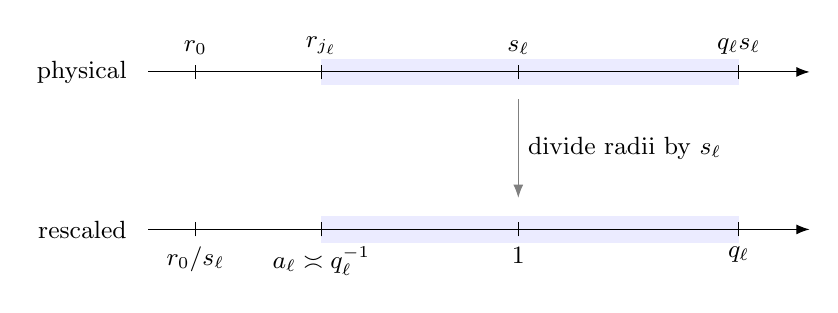
\begin{tikzpicture}[x=1cm,y=1cm,>=Latex,font=\small]
 \fill[blue!8] (2.8,.83) rectangle (8.1,1.17);
 \fill[blue!8] (2.8,-1.17) rectangle (8.1,-.83);
 \draw[->] (.6,1)--(9,1);
 \draw[->] (.6,-1)--(9,-1);
 \node[anchor=east] at (.45,1) {physical};
 \node[anchor=east] at (.45,-1) {rescaled};
 \foreach \x in {1.2,2.8,5.3,8.1}{
   \draw (\x,.91)--(\x,1.09);
   \draw (\x,-1.09)--(\x,-.91);
 }
 \node[above] at (1.2,1.1) {$r_0$};
 \node[above] at (2.8,1.1) {$r_{j_\ell}$};
 \node[above] at (5.3,1.1) {$s_\ell$};
 \node[above] at (8.1,1.1) {$q_\ell s_\ell$};
 \node[below] at (1.2,-1.1) {$r_0/s_\ell$};
 \node[below] at (2.8,-1.1) {$a_\ell\asymp q_\ell^{-1}$};
 \node[below] at (5.3,-1.1) {$1$};
 \node[below] at (8.1,-1.1) {$q_\ell$};
 \draw[->,gray] (5.3,.65)--(5.3,-.6)
   node[midway,right,black] {divide radii by $s_\ell$};
\end{tikzpicture}
\caption{The physical and rescaled radii in
Proposition~\ref{scales:good} (schematic, not to scale).
The same observation index supplies both the comparison on the shaded
annulus and the intermediate subsolution.  Its rescaled inner radius
tends to zero while the outer endpoint tends to infinity.}
\label{fig:scales}
\end{figure}


\begin{proof}
\emph{Inverting the comparison.}
We extract a density approximation from the inverse comparison
\eqref{inp:comparison}.  Fix an integer $q\ge2$ and choose
$h_h>C_{\mathrm{cap}}+1$.  At a point in its comparison band, write
\[
 v=|y|^4H_j(y),\qquad
 t=\left(\frac{|y|^6\mu_j(y)}{k}\right)^{2/3}\ge0.
\]
Choose $0<h_l<h_h$ and $0<\xi<\min\{h_l/16,1\}$, to be decreased below.
The cap and the high implication rule out $t\ge h_h$: taking heights
increasing to $h_h$ would give $v\ge h_h-\xi>C_{\mathrm{cap}}$.
If $h_l<t<h_h$, heights approaching $t$ from below and above give
$|v-t|\le\xi$, and hence $|v_+-t|\le\xi$.
If $t\le h_l$, heights decreasing to $h_l$ in the low implication give
$v\le h_l+\xi$.  This last case includes $t=h_l$ and allows arbitrarily
negative $v$; both $t$ and $v_+$ still lie in $[0,h_l+\xi]$.
Consequently
\[
 k\bigl|t^{3/2}-(v_+)^{3/2}\bigr|
 \le
 \begin{cases}
  \dfrac32 k\sqrt{h_h}\,\xi,& h_l<t<h_h,\\[2pt]
  k(h_l+\xi)^{3/2},& t\le h_l.
 \end{cases}
\]
We may therefore choose $h_l=h_l(q)$ and $\xi=\xi(q)$ so that the
right-hand side is at most $q^{-8}$.  These choices are fixed before the
comparison's smallness threshold for $s$ is imposed.

\emph{Choosing the observation scale.}
For this fixed $q$, take $L_1=q^2$.  The admissibility condition gives
\[
 \frac{r_0}{s_\ell}
 =\eps\bigl(Z_\ell s_\ell^3\bigr)^{-1/3}\longrightarrow0.
\]
Thus, for all sufficiently large $\ell$, the largest dyadic radius not
exceeding $s_\ell/q$ has an index $j<J_\ell$ and satisfies
\[
 \frac{s_\ell}{2q}\le r_j\le\frac{s_\ell}{q}.
\]
Here $j<J_\ell$ follows from $r_{J_\ell}>s_\ell/2$ and $q\ge2$.
Moreover $4L_1r_j\ge2qs_\ell$, so the comparison covers the band
$r_j\le|y|\le qs_\ell$.
The rescaled comparison band thus extends from a radius in
$[1/(2q),1/q]$ to $q$.  On its event we have
\begin{equation}
 H_j(y)\le C_{\mathrm{cap}}|y|^{-4},\qquad
 \bigl|\mu_j(y)-k(H_j(y)_+)^{3/2}\bigr|
 \le q^{-8}|y|^{-6}
 \quad(r_j\le|y|\le qs_\ell).
 \label{scales:physical-band}
\end{equation}
The exceptional probability is at most $C_qs_\ell^{25}$.
The observations and master kernels in
\eqref{inp:observations}--\eqref{inp:packets} are fixed independently of
$L_1,h_l,h_h,\xi$.  Thus this new application of the comparison concerns
exactly the same $\mu_j,H_j$ as the fixed-parameter barrier construction.

\emph{Choosing the stages and retained data.}
Choose strictly increasing stage indices $\ell_q$ so that, for every
$\ell\ge\ell_q$, all the preceding requirements for that fixed $q$ hold,
including $C_qs_\ell^{25}\le1/q$.  On
$\ell_q\le\ell<\ell_{q+1}$ set $q_\ell=q$, and choose the deterministic
index $j_\ell$ just described.  Then $q_\ell\to\infty$,
\eqref{scales:inner-radius} holds, and the comparison events have
probability tending to one.  No bound on the growth of $C_q$, or on the
smallness thresholds as functions of $q$, is needed.

For each system, first choose the conditional-integral versions of the
fields.  At each index $j$, fix an $\mathcal F_j$-measurable full-measure
set on which all its imported identities, regularity properties, and
barrier inequalities hold.  Spatial continuity and a countable dense
family of distributional tests supply the continuum assertions; the
finitely many such sets are fixed before any data are selected.  Intersect
the comparison event at $j_\ell$ with its corresponding valid-data set
and with
\[
 \left\{\int_{\R^3}p_{j_\ell}(y)\,\dd y\le1\right\}.
\]
Call the resulting event $G_\ell$.  The intermediate error estimate
\eqref{inp:barriers} and Markov's inequality give
\[
 \Prob(G_\ell^c)
 \le\frac1{q_\ell}+C\bigl(s_\ell^{32}+s_\ell^\gamma\bigr)
 \longrightarrow0.
\]
In particular the retained-data assertion is pointwise on specified valid
versions, not an assertion left to an exceptional set after a datum is
selected.

\emph{Rescaling.}
Each conditional density has mass
$Z_\ell$, and the Coulomb kernel has degree $-1$, so
\eqref{scales:fields} gives \eqref{scales:mass-field} exactly.
The comparison \eqref{scales:physical-band} gives
\eqref{scales:band}.  Since $f(s^4u)=s^6f(u)$ for $s>0$, rescaling the
imported distributional subsolution inequality gives
\eqref{scales:invariant}, with the barriers
\eqref{scales:barriers}.  The support scales to the ball of radius
$a_\ell$, and on $G_\ell$
\[
 \int_{\R^3}p_\ell(x)\,\dd x
 =s_\ell^3\int_{\R^3}p_{j_\ell}(y)\,\dd y\le s_\ell^3,
\]
which proves \eqref{scales:error}.  The finite-system regularity follows
from the imported barrier regularity and the positive lower bound on
packet widths.  For the field remainder, a bounded integrable density has
a locally Lipschitz Coulomb potential: near the singularity the kernels
$|z|^{-1}$ and $|z|^{-2}$ are integrable in three dimensions, while away
from it both kernels are bounded.  This proves the remaining assertions.
\end{proof}

\section{The unique neutral limiting profile}
\label{prof:section}

Fix one datum in each retained set $G_\ell$ of
Proposition~\ref{scales:good}.  The resulting fields are deterministic;
we use its notation and all its bounds below.  In particular,
$a_\ell\to0$, $q_\ell\to\infty$, and the exact neutral mass identity
\eqref{scales:mass-field} holds, even though
$\lambda_\ell=Z_\ell s_\ell^3\to\infty$ by admissibility.

We first obtain compactness of the signed fields from neutrality
(Lemma~\ref{prof:compactness}), then transfer the positive barrier
(Lemma~\ref{prof:lower}), and finally identify the limit by dilation
(Lemma~\ref{prof:rigidity}).
We do not assume that $F_\ell$ is pointwise nonnegative.

\begin{lemma}[Compactness from the neutral spherical mean]
\label{prof:compactness}
The sequence $(F_\ell)$ is locally uniformly precompact on
$\R^3\setminus\{0\}$.  Every locally uniform subsequential limit $F$
is locally Lipschitz and satisfies
\begin{equation}
\label{prof:limit-equation}
 \Delta F=f(F),\qquad F(x)\le C_{\rm cap}|x|^{-4},\qquad
 \frac1{4\pi}\int_{\mathbb S^2}F(d\omega)\,\dd\omega\ge0
 \quad(d>0).
\end{equation}
Along the same subsequence,
$\sigma_\ell\to k(F_+)^{3/2}$ locally uniformly away from zero.
Moreover, there is a constant $C_*$, depending only on $C_{\rm cap}$
and $k$, such that
\begin{equation}
\label{prof:absolute}
 |F(x)|\le C_*|x|^{-4}\qquad(x\ne0).
\end{equation}
The family of dilates $\{D^4F(D\,\cdot):D>0\}$ is also locally
uniformly precompact away from zero.
\end{lemma}

\begin{proof}
Newton's spherical-average identity is
\[
 \frac1{4\pi}\int_{\mathbb S^2}\frac{\dd\omega}{|d\omega-z|}
 =\frac1{\max(d,|z|)}.
\]
It follows either by direct integration in the angle with $z$, or by
the mean-value property inside and outside the sphere.  Applying it
to \eqref{scales:mass-field} and using the exact equality of the nuclear
coefficient and total density mass gives
\begin{equation}
\label{prof:mean}
 \overline F_\ell(d):=
 \frac1{4\pi}\int_{\mathbb S^2}F_\ell(d\omega)\,\dd\omega
 =\int_{|z|>d}\left(\frac1d-\frac1{|z|}\right)
                    \sigma_\ell(z)\,\dd z\ge0.
\end{equation}
All these integrals are finite for each $\ell$.  No upper bound on
$\lambda_\ell$ is needed.

Fix an annulus $\alpha\le |x|\le\beta$ with $0<\alpha<\beta<\infty$.
For large $\ell$, it lies in the band of \eqref{scales:band}.  The cap
and \eqref{prof:mean} imply, for every radius in this annulus,
\begin{equation}
\label{prof:sphere-lone}
 \int_{\mathbb S^2}|F_\ell(d\omega)|\,\dd\omega
 =2\int_{\mathbb S^2}(F_\ell(d\omega))_+\,\dd\omega
    -\int_{\mathbb S^2}F_\ell(d\omega)\,\dd\omega
 \le 8\pi C_{\rm cap}d^{-4}.
\end{equation}
Radial integration therefore bounds the full $L^1$ norm of $F_\ell$
on the annulus.  Equation~\eqref{scales:band} also bounds
$\sigma_\ell$ uniformly there.

Here is the local estimate we shall use twice.  Take a ball $Q$ whose
closure stays away from zero, and a larger fixed annulus containing
its closure.  The localized potential
\[
 P_\ell=K*(\sigma_\ell\1_Q)
\]
has uniformly bounded values and first derivatives: this follows
from the density bound and the integrability of $|z|^{-1}$ and
$|z|^{-2}$ on bounded subsets of $\R^3$.  Since
$\Delta F_\ell=4\pi\sigma_\ell$ on $Q$, the function
$h_\ell=F_\ell+P_\ell$ is distributionally harmonic there.  Its
$L^1(Q)$ norm is bounded by \eqref{prof:sphere-lone} and the bound on
$P_\ell$.  On every smaller concentric ball, harmonic interior
estimates bound $h_\ell$ and its gradient by this $L^1$ norm.  For
completeness, convolution with a fixed smooth radial averaging kernel
reproduces a harmonic function in the interior; differentiating that
convolution gives these bounds.  The same argument applies to
continuous distributionally harmonic functions, by first mollifying
on interior sets.  Subtracting $P_\ell$ gives uniform local value and
Lipschitz bounds for $F_\ell$.

A covering by such balls, followed by a diagonal
Arzel\`a--Ascoli argument, gives local uniform precompactness and a
locally Lipschitz limit.  The error in \eqref{scales:band} tends
uniformly to zero on every fixed compact annulus, so
$\sigma_\ell\to k(F_+)^{3/2}$ there.  Passing to distributions, to the
cap, and to the spherical averages proves
\eqref{prof:limit-equation}.

To compare with $U_\ell$ on large spheres, we next strengthen the
one-sided cap to an absolute bound for $F$.
For $D>0$ set $F^{(D)}(x)=D^4F(Dx)$.  The equation, cap, and
nonnegative spherical means in \eqref{prof:limit-equation} are
invariant under this dilation.  In particular, on a fixed annulus
the same argument as in \eqref{prof:sphere-lone} bounds the $L^1$
norm of every $F^{(D)}$, while the source
$k(F^{(D)}_+)^{3/2}$ is uniformly bounded by the cap.  The local
estimate just proved is therefore uniform in $D$.  It yields both
precompactness of the dilates and a uniform bound
$|F^{(D)}(\omega)|\le C_*$ for $|\omega|=1$.  Writing $x=D\omega$
proves \eqref{prof:absolute}.
\end{proof}

\begin{lemma}[Transfer of the positive barrier]
\label{prof:lower}
Every limit $F$ in Lemma~\ref{prof:compactness} satisfies
\begin{equation}
\label{prof:positive}
 B|x|^{-4}\le F(x)\le C_{\rm cap}|x|^{-4}\qquad(x\ne0).
\end{equation}
\end{lemma}

\begin{proof}
We compare the barrier and the screened field on a fixed ball after
subtracting a Coulomb correction that vanishes away from the origin.
Work along the subsequence converging to $F$.  Fix $S>0$; eventually
$a_\ell<S<q_\ell$.  Define
\begin{equation}
\label{prof:correction}
 e_\ell(x)=q_\ell^{-8}|x|^{-6}
                    \1_{\{a_\ell\le|x|\le S\}},
 \qquad L_\ell=K*(p_\ell+e_\ell)\ge0.
\end{equation}
Subtracting the Poisson equation for $F_\ell$ from
\eqref{scales:invariant} cancels the nucleus and the entire inner
density source.  Since
$4\pi\sigma_\ell\le f(F_\ell)+4\pi e_\ell$ on
$a_\ell\le|x|<S$ and $\Delta(-L_\ell)=4\pi(p_\ell+e_\ell)$, the
result is
\begin{equation}
\label{prof:comparison-inequality}
 \Delta(U_\ell-F_\ell-L_\ell)
 \ge \1_{\{|x|\ge a_\ell\}}
                  \bigl(f(U_\ell)-f(F_\ell)\bigr)
 \quad\hbox{in }B(0,S).
\end{equation}
This is an inequality on the whole ball, including the origin and
the sphere $|x|=a_\ell$; no restriction or differentiation across an
interface has been made.

Put
\[
 c_S=(C_{\rm inv}+C_*+1)S^{-4}.
\]
Uniform convergence on $|x|=S$, the bound
\eqref{prof:absolute}, the upper barrier in
\eqref{scales:barriers}, and $L_\ell\ge0$ give, for large $\ell$,
\[
 U_\ell-F_\ell-L_\ell<c_S\qquad\hbox{on }|x|=S.
\]
We justify the comparison throughout the ball.  The difference
\[
 W_\ell=U_\ell-F_\ell-L_\ell-c_S
       =(U_\ell-\lambda_\ell K)+K*\sigma_\ell-L_\ell-c_S
\]
extends continuously and locally in $H^1$ across zero.  Indeed, the
first term is locally Lipschitz by hypothesis.  The other potentials
have bounded integrable densities for each fixed $\ell$, and thus
locally bounded gradients.  In the case of $L_\ell$ the density is
also compactly supported.  These bounds need not be uniform in
$\ell$.

The strict boundary inequality implies that $(W_\ell)_+$ has compact
support in $B(0,S)$ and belongs to $H^1_0(B(0,S))$.  It may therefore
be used in \eqref{prof:comparison-inequality}, by approximation with
nonnegative smooth tests in $H^1$.  The right side is bounded on
this fixed ball for this fixed $\ell$, since its reaction is cut off
at the positive radius $a_\ell$.  On the positive set of $W_\ell$
outside that radius, we have $U_\ell>F_\ell$, because
$L_\ell+c_S>0$.  Monotonicity of $f$ consequently gives
\[
 -\int_{B(0,S)}|\nabla(W_\ell)_+|^2\,\dd x
 \ge\int_{B(0,S)}\1_{\{|x|\ge a_\ell\}}
       \bigl(f(U_\ell)-f(F_\ell)\bigr)(W_\ell)_+\,\dd x
 \ge0.
\]
It follows that $(W_\ell)_+=0$, or equivalently
\begin{equation}
\label{prof:comparison}
 U_\ell\le F_\ell+L_\ell+c_S\qquad\hbox{in }B(0,S).
\end{equation}

For each fixed $x$ with $0<|x|<S$, we next show that
$L_\ell(x)\to0$.  For large $\ell$, the support and mass bound in
\eqref{scales:error} imply
\[
 (K*p_\ell)(x)\le \frac{2s_\ell^3}{|x|}\longrightarrow0.
\]
The other source has small total mass:
\[
 \int e_\ell\,\dd x
 =\frac{4\pi}{3}q_\ell^{-8}(a_\ell^{-3}-S^{-3})
 \le\frac{32\pi}{3}q_\ell^{-5}\longrightarrow0.
\]
On the fixed ball $B(x,|x|/4)$ its density is at most
$C_xq_\ell^{-8}$.  Integrability of the Coulomb kernel bounds its
potential contribution there by $C_xq_\ell^{-8}$; on the complement
the kernel is at most $4/|x|$, so the contribution is at most
$(4/|x|)\int e_\ell$.  Hence $L_\ell(x)\to0$.

Now \eqref{prof:comparison} and the lower barrier give
\[
 F(x)+c_S\ge B|x|^{-4}.
\]
The argument holds for every fixed $S>|x|$ along the same convergent
subsequence.  Letting $S\to\infty$ proves the lower bound in
\eqref{prof:positive}; the upper bound was already known.
\end{proof}

The next rigidity statement also follows from Solovej's nonradial
Sommerfeld estimate \cite[Lemma~4.4 and Remark~4.5]{Solovej2003}:
in that estimate, take inner radius zero and use the positive
two-sided $|x|^{-4}$ bounds.  We retain a direct dilation proof to
make the precise compactness and contact argument explicit.

\begin{lemma}[Rigidity of a positive comparable profile]
\label{prof:rigidity}
Let $F$ be a continuous distributional solution of
$\Delta F=4\pi kF^{3/2}$ on $\R^3\setminus\{0\}$, and suppose
\[
 B|x|^{-4}\le F(x)\le C|x|^{-4}\qquad(x\ne0)
\]
for constants $0<B\le C<\infty$.  Then
\begin{equation}
\label{prof:homogeneous}
 F(x)=A_*|x|^{-4},\qquad
 A_*=\left(\frac{12}{4\pi k}\right)^2=\frac{81\pi^2}{8}.
\end{equation}
No radiality assumption is required.
\end{lemma}

\begin{proof}
The local potential and harmonic estimates in
Lemma~\ref{prof:compactness} apply uniformly to the dilates
$F^{(D)}(x)=D^4F(Dx)$: their values and their sources are bounded on
every fixed compact annulus.  Thus the dilates are locally uniformly
precompact, with locally Lipschitz limits satisfying the same
equation.

Write
\[
 b=\sup_{x\ne0}|x|^4F(x),\qquad
 h=\inf_{x\ne0}|x|^4F(x),
 \qquad 0<h\le b<\infty.
\]
Choose $x_n$ with $|x_n|^4F(x_n)\to b$, and let
$D_n=|x_n|$, $\omega_n=x_n/|x_n|$.  After passing to a subsequence,
$F^{(D_n)}\to v$ locally uniformly and $\omega_n\to\omega\in\mathbb S^2$.
Local equicontinuity gives
\[
 v(x)\le b|x|^{-4}\quad(x\ne0),\qquad v(\omega)=b.
\]
The equation passes to the limit because its reaction is continuous
and locally uniformly bounded.  Since
$\Delta |x|^{-4}=12|x|^{-6}$ in three dimensions, this contact implies
\begin{equation}
\label{prof:upper-contact}
 4\pi k b^{3/2}\le12b.
\end{equation}
Here is a weak proof of the contact assertion.  If the inequality
failed, the continuous function $g=v-b|x|^{-4}$ would satisfy
$g\le0$, $g(\omega)=0$, and $\Delta g\ge\delta>0$ on a sufficiently
small ball about $\omega$.  For $0<\eta<\delta/6$, the function
$g-\eta|x-\omega|^2$ is weakly subharmonic there, equals zero at the
center, and is strictly negative on the boundary.  Choose a level
strictly between its boundary maximum and zero.  Testing its
Laplacian with the positive part above that level, as in the proof of
Lemma~\ref{prof:lower}, contradicts the value at the center.
This proves \eqref{prof:upper-contact} without a classical second
derivative assumption.

Dilating instead along points approaching the infimum gives a limit
$v\ge h|x|^{-4}$ with equality at a unit point.  If
$4\pi k h^{3/2}<12h$, the same argument applies to
$h|x|^{-4}-v$, whose Laplacian is then strictly positive near its zero
maximum.  Consequently
\[
 4\pi k h^{3/2}\ge12h.
\]
Together with \eqref{prof:upper-contact}, this gives
$b\le A_*\le h$.  Since $h\le b$, both extrema equal $A_*$, proving
\eqref{prof:homogeneous}.  The argument allows $D_n$ to tend to zero,
to infinity, or to neither; no extremum of the original field had to
be attained.
\end{proof}

\begin{proposition}[Convergence of the selected fields]
\label{prof:limit}
For every choice of one retained datum at each index,
\[
 F_\ell(x)\longrightarrow A_*|x|^{-4},\qquad
 \sigma_\ell(x)\longrightarrow
 \rho_*(x):=kA_*^{3/2}|x|^{-6}
\]
locally uniformly on $\R^3\setminus\{0\}$.
\end{proposition}

\begin{proof}
Lemma~\ref{prof:compactness} gives a locally uniformly convergent
subsequence of every subsequence.  Its limit satisfies the positive
bounds of Lemma~\ref{prof:lower}, so Lemma~\ref{prof:rigidity}
identifies it as $A_*|x|^{-4}$.  Uniqueness of every subsequential
limit proves convergence of the full sequence.  The density
convergence follows from \eqref{scales:band}.
\end{proof}

\begin{corollary}[Uniformity on the retained data]
\label{prof:uniform}
For each fixed compact annulus $\mathcal A\subset\R^3\setminus\{0\}$,
\[
 \sup_{\theta\in G_\ell}
 \left\|\sigma_\ell(\theta,\,\cdot)-\rho_*\right\|_{C(\mathcal A)}
 \longrightarrow0.
\]
The corresponding assertion holds for
$F_\ell(\theta,\,\cdot)-A_*|\cdot|^{-4}$.
\end{corollary}

\begin{proof}
If either assertion failed, there would be a positive discrepancy
along a subsequence and a choice of one datum from each corresponding
$G_\ell$ realizing at least half that discrepancy.  Those selected
fields satisfy all the same deterministic hypotheses, contradicting
Proposition~\ref{prof:limit}.  This argument uses no measurable
selection: uniformity is a deterministic assertion about all the
retained data, after the conditional versions have been fixed.
\end{proof}

\section{Expected electron tails and the radius limits}\label{sec:tails}

Fix any admissible sequence from~\eqref{scales:admissible}, with
arbitrary normalized neutral ground states $\Psi_\ell$ at charges
$Z_\ell$. Use the indices $j_\ell$ and retained events $G_\ell$ of
Proposition~\ref{scales:good}.
Throughout this section, $\sigma_\ell$ is the conditional-integral
version from~\eqref{scales:fields} on the full data space, and
expectations are taken under the original enlarged law.
Thus $\Prob(G_\ell)\to1$, and
Corollary~\ref{prof:uniform} gives uniform convergence of
$\sigma_\ell$ to
\[
 \rho_*(x)=kA_*^{3/2}|x|^{-6}
\]
on each fixed compact annulus, uniformly over the data in $G_\ell$.
We now pass from these conditional densities to expected counts of
raw electron positions. Every fixed sphere has zero expected raw
count, since each one-electron marginal is absolutely continuous.

For $0<a<b<\infty$, write
\[
 \mathcal A(a,b)=\{x:a<|x|<b\},\qquad
 N_\ell(a,b)=\#\{i:a s_\ell<|x_i|<b s_\ell\},
\]
and let
\[
 P_\ell(a,b)=\sum_{i=1}^{Z_\ell}
       \int_{s_\ell\mathcal A(a,b)}\mathcal K_{x_i}(y)\dd y
\]
be the mass of the smoothing packets in the same physical annulus.
The packets and their widths are those of~\eqref{inp:packets} for the
$\ell$th system. Conditional integration and a change of variables give
\begin{equation}\label{tail:conditional-mass}
 \int_{\mathcal A(a,b)}\sigma_\ell(x)\dd x
   =s_\ell^3\E\bigl[P_\ell(a,b)\mid\mathcal F_{j_\ell}\bigr].
\end{equation}

\begin{lemma}[Packet supports]\label{tail:packets}
For each fixed $0<a<b<\infty$, all sufficiently large $\ell$ satisfy
\begin{equation}\label{tail:localization}
 P_\ell(a,b)\le N_\ell(a/2,2b)
\end{equation}
for every raw configuration. Moreover, for every fixed
$0<\eta<\min\{a,(b-a)/2\}$, all sufficiently large $\ell$ satisfy
\begin{equation}\label{tail:sandwich}
 P_\ell(a+\eta,b-\eta)
    \le N_\ell(a,b)
    \le P_\ell(a-\eta,b+\eta)
\end{equation}
for every raw configuration.
\end{lemma}

\begin{proof}
Abbreviate $s=s_\ell$ and $r_0=\eps Z_\ell^{-1/3}$, and set
$\delta_s=c_1s^w\to0$. If a packet centered at $z$ has $|z|\ge r_0$,
then its width obeys $t_z\le\delta_s|z|$. Consequently
\begin{equation}\label{tail:relative-support}
 \mathcal K_z(y)\ne0
 \quad\Longrightarrow\quad
 (1-\delta_s)|z|\le |y|\le(1+\delta_s)|z|.
\end{equation}
This estimate holds also for arbitrarily distant centers. If instead
$|z|<r_0$, its packet is contained in the ball of radius
\[
 r_0+c_1r_0^{1+w}=o(s),
\]
because $r_0/s=\eps(Z_\ell s_\ell^3)^{-1/3}\to0$. Such packets
therefore cannot meet any fixed annulus $s\mathcal A(a,b)$ for large
$\ell$. For the remaining packets, \eqref{tail:relative-support}
shows that a packet meeting this annulus has center in
$s\mathcal A(a/2,2b)$ once $\delta_s$ is small. Each packet has mass
one, proving~\eqref{tail:localization}.

The same inequalities show that every packet meeting the contracted
annulus $s\mathcal A(a+\eta,b-\eta)$ has its center in
$s\mathcal A(a,b)$. Conversely, every packet whose center lies in
$s\mathcal A(a,b)$ is entirely contained in the enlarged annulus
$s\mathcal A(a-\eta,b+\eta)$. For example,
$\delta_s<\eta/b$ suffices for these inclusions once the clamped
packets have been excluded. Summing the mass-one packets proves both
inequalities in~\eqref{tail:sandwich}.
\end{proof}

\begin{lemma}[Expected annular mass]\label{tail:annular}
For every fixed $0<a<b<\infty$,
\begin{align}
 \E\int_{\mathcal A(a,b)}\sigma_\ell(x)\dd x
       &\longrightarrow \int_{\mathcal A(a,b)}\rho_*(x)\dd x,
          \label{tail:smoothed-annulus}\\
 s_\ell^3\E N_\ell(a,b)
       &\longrightarrow \int_{\mathcal A(a,b)}\rho_*(x)\dd x.
          \label{tail:raw-annulus}
\end{align}
\end{lemma}

\begin{proof}
Put $Y_\ell=\int_{\mathcal A(a,b)}\sigma_\ell$ and
$X_\ell=N_\ell(a/2,2b)$. Equations~\eqref{tail:conditional-mass}
and~\eqref{tail:localization}, followed by conditional Jensen, give
\[
 0\le Y_\ell\le s_\ell^3\E[X_\ell\mid\mathcal F_{j_\ell}],
 \qquad
 \|Y_\ell\|_2\le s_\ell^3\|X_\ell\|_2.
\]
The annular count bound~\eqref{inp:counts}, with the common offset
$D_0$ and $s_\ell<1$, therefore yields
\begin{equation}\label{tail:uniform-integrability}
 \|Y_\ell\|_2
 \le C\bigl(1+\sqrt{D_0}\,s_\ell^{7/2}\bigr)\le C'.
\end{equation}
In particular, for the actual complement of the retained event,
\[
 \E\bigl[Y_\ell\1_{G_\ell^c}\bigr]
       \le C'\Prob(G_\ell^c)^{1/2}\longrightarrow0.
\]
No independence of $G_\ell$ from the conditional fields is required.
On $G_\ell$, Corollary~\ref{prof:uniform} implies that $Y_\ell$
converges to $\int_{\mathcal A(a,b)}\rho_*$ uniformly over all retained
data. Since $\Prob(G_\ell)\to1$, this proves
\eqref{tail:smoothed-annulus}.

Taking expectations in~\eqref{tail:conditional-mass} gives
$\E Y_\ell=s_\ell^3\E P_\ell(a,b)$. Apply
\eqref{tail:smoothed-annulus} to the contracted and enlarged annuli
in~\eqref{tail:sandwich}. It follows that
\begin{align*}
 \int_{\mathcal A(a+\eta,b-\eta)}\rho_*
  &\le \liminf_{\ell\to\infty}s_\ell^3\E N_\ell(a,b)\\
  &\le \limsup_{\ell\to\infty}s_\ell^3\E N_\ell(a,b)
   \le \int_{\mathcal A(a-\eta,b+\eta)}\rho_*.
\end{align*}
Letting $\eta\downarrow0$ proves~\eqref{tail:raw-annulus}, because
$\rho_*$ is continuous and integrable on a neighborhood of the fixed
closed annulus.
\end{proof}

\begin{lemma}[Exterior tightness]\label{tail:tightness}
There is a constant $C$, independent of the fixed number $M>0$, such
that every admissible sequence satisfies
\begin{equation}\label{tail:tightness-bound}
 \limsup_{\ell\to\infty}s_\ell^3
      \E\#\{i:|x_i|>Ms_\ell\}\le CM^{-3}.
\end{equation}
\end{lemma}

\begin{proof}
For fixed $M$, eventually $Ms_\ell<1$. Cover the region between
$Ms_\ell$ and $1$ by shells $u<|x|<2u$, with
$u=2^pMs_\ell<1$ and $p=0,1,\ldots$. The annular bound
\eqref{inp:counts}, applied with the fixed shape $(1,2)$, gives
\[
 \E\#\{i:u<|x_i|<2u\}
 \le C\bigl(u^{-3}+\sqrt{D_0u}\bigr)\le C_Du^{-3}
 \qquad(0<u<1).
\]
The expected raw mass outside radius $1$ is bounded by the other
estimate in~\eqref{inp:counts}. Summing the geometric series, and
allowing the last shell to overlap this exterior region, gives
\[
 s_\ell^3\E\#\{i:|x_i|>Ms_\ell\}
 \le C_D M^{-3}\sum_{p=0}^{\infty}2^{-3p}+Cs_\ell^3.
\]
The constants depend only on the fixed count estimates and $D_0$;
they do not depend on $M$. Taking the upper limit proves the claim.
\end{proof}

\begin{theorem}[Expected exterior asymptotic]\label{tail:asymptotic}
Along every admissible sequence, with arbitrary normalized neutral
ground states, for each fixed $a>0$,
\begin{equation}\label{tail:asymptotic-equation}
 s_\ell^3\int_{|y|>as_\ell}\rho_{\Psi_\ell}(y)\dd y
       \longrightarrow \frac{b_{\mathrm{TF}}^3}{a^3}.
\end{equation}
\end{theorem}

\begin{proof}
Fix $M>a$. Lemma~\ref{tail:annular} gives convergence on
$\mathcal A(a,M)$, whereas Lemma~\ref{tail:tightness} bounds the
remaining exterior mass after rescaling by $CM^{-3}$. Thus, with
$T_\ell(r)=\int_{|y|>r}\rho_{\Psi_\ell}(y)\dd y$,
\begin{align*}
 \liminf_{\ell\to\infty}s_\ell^3T_\ell(as_\ell)
   &\ge \int_{\mathcal A(a,M)}\rho_*,\\
 \limsup_{\ell\to\infty}s_\ell^3T_\ell(as_\ell)
   &\le \int_{\mathcal A(a,M)}\rho_*+CM^{-3}.
\end{align*}
Let $M\to\infty$. The limiting density is integrable outside every
positive radius, and
\[
 \int_{|x|>a}\rho_*(x)\dd x
 =\frac{4\pi kA_*^{3/2}}{3a^3}
 =\frac{4A_*}{a^3}
 =\frac{b_{\mathrm{TF}}^3}{a^3},
\]
using $4\pi kA_*^{1/2}=12$ and $4A_*=81\pi^2/2$.
This proves~\eqref{tail:asymptotic-equation}.
\end{proof}

\begin{proof}[Proof of Theorem~\ref{intro:main}]
For each sufficiently large integer $m$, put $s=m^{-1/3}$ and choose
a finite integer
\[
 Z_{\min}(m)\ge
 \max\{m+1,\,Z_{\mathrm{bar}}(m^{-1/3}),\,m^{4/3}\}.
\]
The barrier threshold is uniform over normalized ground states.
Consequently every sequence with $m\to\infty$ and
$Z\ge Z_{\min}(m)$ is admissible: in particular,
$Zs^3\ge m^{1/3}\to\infty$.

Fix $0<a_-<b_{\mathrm{TF}}<a_+$. We claim that, for all sufficiently large
integers $m$, all integers $Z\ge Z_{\min}(m)$, and every normalized
neutral ground state $\Psi$ of charge $Z$,
\begin{equation}\label{tail:strict-bracket}
 \int_{|y|>a_-m^{-1/3}}\rho_\Psi(y)\dd y>m,
 \qquad
 \int_{|y|>a_+m^{-1/3}}\rho_\Psi(y)\dd y<m.
\end{equation}
Otherwise choose strictly increasing violating integers $m_\ell$,
charges $Z_\ell\ge Z_{\min}(m_\ell)$, and corresponding ground states
$\Psi_\ell$. With $s_\ell=m_\ell^{-1/3}$ this is an admissible
sequence. Theorem~\ref{tail:asymptotic}, applied separately at $a_-$
and $a_+$, gives normalized tail limits
$b_{\mathrm{TF}}^3/a_-^3>1$ and $b_{\mathrm{TF}}^3/a_+^3<1$. Hence both
inequalities in~\eqref{tail:strict-bracket} eventually hold on this
sequence, a contradiction. This argument includes arbitrary choices
of the ground states at the selected charges.

The tail mass is nonincreasing in its radius and tends to zero, so
the set defining $R_m(\Psi)$ is nonempty. The first inequality in
\eqref{tail:strict-bracket} excludes every radius at most
$a_-m^{-1/3}$ from that set; the second places $a_+m^{-1/3}$ in the
set. Thus
\begin{equation}\label{tail:radius-bracket}
 a_-\le m^{1/3}R_m(\Psi)\le a_+
\end{equation}
for all the states and charges just specified.

Now fix any family $(\Psi_Z)_{Z\ge1}$ of normalized neutral ground
states. For each fixed sufficiently large integer $m$, removing the
finite prefix $Z<Z_{\min}(m)$ changes neither the inner upper limit
nor the inner lower limit. Both
\[
 m^{1/3}\limsup_{\substack{Z\to\infty\\Z>m}}R_m(\Psi_Z)
 \quad\hbox{and}\quad
 m^{1/3}\liminf_{\substack{Z\to\infty\\Z>m}}R_m(\Psi_Z)
\]
therefore lie between $a_-$ and $a_+$. Finally let $m\to\infty$ and
squeeze with arbitrary $a_-<b_{\mathrm{TF}}<a_+$. This proves both asserted
limits. No convergence in $Z$ at fixed $m$ is used.
\end{proof}

\appendix
\section{Foundation providers and parameter choices}\label{sec:interface}

Section~\ref{sec:inputs} states the complete hypotheses used in this
article.  Their proofs are in the separate foundation companion
\emph{Uniform excess charge for Coulomb molecules and the outer radius
of neutral atoms} \cite{OuterRadius}.  This appendix identifies the
provider results and explains the compatibility of their parameter
choices.  All inputs use two spin states, kinetic operator $-\Delta/2$,
and the constants in \eqref{intro:constants}.

\paragraph{States and raw counts.}
Ground-state existence comes from \FoundationBinding\ of
\cite{OuterRadius}, and sector monotonicity from \FoundationMonotonicity;
the bounded neutral offset uses \FoundationOffset.  The annular $L^2$ bound in
\cref{inp:energy-counts} is \FoundationCounts, and the unit-radius
exterior bound follows from \FoundationDeficit\ with $t=4$ and exactly
$Z$ electrons.  These inputs apply uniformly to every normalized neutral
ground state, not only to a selected family of states.

\paragraph{Common observations and conditional versions.}
\FoundationObservations\ of \cite{OuterRadius} supply the observation
law and likelihood-integral versions used in
\eqref{inp:observations}--\eqref{inp:mass-poisson}.  In particular, the
same master packets define all the conditional densities.  Their exact
mass, Poisson and tower identities and finite-system regularity hold
on fixed full-measure sets.  The derivative and local Lipschitz bounds
need not be uniform in $Z$.

\paragraph{Comparison and intermediate subsolutions.}
\FoundationComparison\ of \cite{OuterRadius} supplies
\cref{inp:comparison-prop}: arbitrary fixed annular width and accuracy,
a universal upper cap, and an exceptional probability of order
$r_j^{25}$.  \FoundationIntermediate\ supplies
\cref{inp:barrier-prop} at every intermediate index, with constants
independent of the number of scales.  Its expected error bound controls
every prefix, as explained after \eqref{inp:barriers}.  At the terminal
index the sigma-field is trivial, so the same bound is deterministic.
The almost-sure subsolution assertions do not make the comparison event
a full-measure event.

\paragraph{Order of choices.}
First fix the kernel and propagation constants, including $\eps$ and
the positive barrier coefficient $B$.  Then fix a requested comparison
band and accuracy, make $s$ sufficiently small for that comparison and
the fixed barrier construction, and take $Z$ above the finite threshold
$Z_{\mathrm{bar}}(s)$.  This threshold includes $Z\ge Z_0$ and
$2\eps Z^{-1/3}\le s$.  Changing $L_1,h_l,h_h,\xi$ changes the comparison
event and its smallness requirement, not the observations, packets,
conditional fields, or fixed barrier construction.

These two uniformities serve different purposes.  The common fields
allow Section~\ref{sec:scales} to improve the comparison accuracy along
a slow diagonal while retaining the same subsolutions.  Uniformity in
the neutral ground state allows Section~\ref{sec:tails} to turn the
result along every admissible sequence into a finite-charge threshold
valid for all such states.  No rate of growth for
$Z_{\mathrm{bar}}(s)$ is asserted or used.

\begin{thebibliography}{SSS90}

\bibitem[FNV18]{FrankNamVanDenBosch2018}
R.~L.~Frank, P.~T.~Nam, and H.~Van Den Bosch,
\emph{The ionization conjecture in Thomas--Fermi--Dirac--von Weizs\"acker theory},
Communications on Pure and Applied Mathematics \textbf{71} (2018),
no.~3, 577--614.
\href{https://doi.org/10.1002/cpa.21717}{doi:10.1002/cpa.21717}.
Also \href{https://arxiv.org/abs/1606.07355}{arXiv:1606.07355}.

\bibitem[K17]{Kehle2017}
C.~Kehle,
\emph{The maximal excess charge for a family of density-matrix-functional
theories including Hartree--Fock and M\"uller theories},
Journal of Mathematical Physics \textbf{58} (2017), no.~1, 011901.
\href{https://doi.org/10.1063/1.4973850}{doi:10.1063/1.4973850}.
Also \href{https://arxiv.org/abs/1609.06272}{arXiv:1609.06272}.

\bibitem[LS77]{LiebSimon1977}
E.~H.~Lieb and B.~Simon,
\emph{The Thomas--Fermi theory of atoms, molecules and solids},
Advances in Mathematics \textbf{23} (1977), no.~1, 22--116.
\href{https://doi.org/10.1016/0001-8708(77)90108-6}{doi:10.1016/0001-8708(77)90108-6}.

\bibitem[Ob]{EnergyPart}
OpenAI,
\emph{Generalized ionization energies for full Coulomb atoms},
OpenAI Math Release preprint
\href{https://github.com/openai/math/blob/main/preprints/Generalized-ionization-energies-for-full-Coulomb-atoms-September-24-2026/paper.pdf}{OAI:Generalized-ionization-energies-for-full-Coulomb-atoms-September-24-2026},
2026.

\bibitem[Oa]{OuterRadius}
OpenAI,
\emph{Uniform excess charge for Coulomb molecules and the outer radius of neutral atoms},
OpenAI Math Release preprint
\href{https://github.com/openai/math/blob/main/preprints/Uniform-excess-charge-for-Coulomb-molecules-and-the-outer-radius-of-neutral-atoms-September-24-2026/paper.pdf}{OAI:Uniform-excess-charge-for-Coulomb-molecules-and-the-outer-radius-of-neutral-atoms-September-24-2026},
2026.

\bibitem[SSS90]{SecoSigalSolovej1990}
L.~A.~Seco, I.~M.~Sigal, and J.~P.~Solovej,
\emph{Bound on the ionization energy of large atoms},
Communications in Mathematical Physics \textbf{131} (1990),
no.~2, 307--315.
\href{https://doi.org/10.1007/BF02161416}{doi:10.1007/BF02161416}.

\bibitem[S03]{Solovej2003}
J.~P.~Solovej,
\emph{The ionization conjecture in Hartree--Fock theory},
Annals of Mathematics (2) \textbf{158} (2003), no.~2, 509--576.
\href{https://doi.org/10.4007/annals.2003.158.509}{doi:10.4007/annals.2003.158.509}.

\bibitem[S16]{Solovej2016}
J.~P.~Solovej,
\emph{A new look at Thomas--Fermi theory},
Molecular Physics \textbf{114} (2016), nos.~7--8, 1036--1040.
\href{https://doi.org/10.1080/00268976.2015.1130273}{doi:10.1080/00268976.2015.1130273}.
Also \href{https://arxiv.org/abs/1601.00497}{arXiv:1601.00497}.

\end{thebibliography}

\end{document}
